\documentclass[10pt,a4paper,UTF8]{ctexart}

\linespread{1.5}
\usepackage{geometry}%用于设置上下左右页边距
	\geometry{left=2.5cm,right=2.5cm,top=3.2cm,bottom=2.7cm}
\usepackage{xeCJK,amsmath,paralist,enumerate,booktabs,multirow,graphicx,subfig,setspace,listings,lastpage,hyperref}
\usepackage{amsthm, amssymb, bm, color, framed, graphicx, hyperref, mathrsfs}
\usepackage{mathrsfs}  
	\setlength{\parindent}{2em}
	\lstset{language=Matlab}%
\usepackage{fancyhdr}
\usepackage{graphicx}
\usepackage{subfloat}
\usepackage{listings}
\usepackage{xcolor}
\usepackage{float}
\usepackage{paralist}
\usepackage{setspace}
\usepackage{titlesec}
\usepackage{enumitem}
\usepackage{hyperref}
\usepackage{multirow}
\usepackage{threeparttable}
\usepackage{tcolorbox}
\usepackage{tabularx}
\usepackage{ulem}
\usepackage{longtable}
\usepackage{multicol}
\usepackage{pifont}
\usepackage{lipsum}
\usepackage{microtype}
\usepackage{wrapfig}
\usepackage[absolute,overlay]{textpos}
\usepackage{makecell}
\usepackage{soul}
\usepackage{xeCJKfntef}


\setmainfont{Times New Roman}[SmallCapsFont=TeX Gyre Termes:+smcp]

\hypersetup{
	colorlinks=true,
	linkcolor=black,
	urlcolor=black
}

\setenumerate{partopsep=0pt,topsep=0pt,itemsep=-2pt,leftmargin=2em}
\setitemize{itemsep=-2pt,partopsep=0pt,topsep=0pt,leftmargin=2em}

\titlespacing*{\section}{0pt}{3pt}{3pt}
\titlespacing*{\subsection}{0pt}{2pt}{2pt}
\titlespacing*{\subsubsection}{0pt}{1pt}{1pt}
\titlespacing*{\paragraph}{0pt}{0pt}{0pt}

\ctexset{secnumdepth=4,tocdepth=4}
\setlength{\parindent}{0pt}
\setstretch{1.35}


\setCJKmainfont[BoldFont={FZHei-B01},ItalicFont={FZKai-Z03}]{FZShuSong-Z01} 
\setCJKsansfont[BoldFont={FZHei-B01}]{FZKai-Z03} 
\setCJKmonofont[BoldFont={FZHei-B01}]{FZFangSong-Z02}
\setCJKfamilyfont{zhsong}{FZShuSong-Z01} 
\setCJKfamilyfont{zhhei}{FZHei-B01} 
\setCJKfamilyfont{zhkai}[BoldFont={FZHei-B01}]{FZKai-Z03} 
\setCJKfamilyfont{zhfs}[BoldFont={FZHei-B01}]{FZFangSong-Z02} 
\renewcommand*{\songti}{\CJKfamily{zhsong}} 
\renewcommand*{\heiti}{\CJKfamily{zhhei}} 
\renewcommand*{\kaishu}{\CJKfamily{zhkai}} 
\renewcommand*{\fangsong}{\CJKfamily{zhfs}}


\definecolor{mKeyword}{RGB}{0,0,255}          % bule
\definecolor{mString}{RGB}{160,32,240}        % purple
\definecolor{mComment}{RGB}{34,139,34}        % green
\definecolor{mNumber}{RGB}{128,128,128} 

\lstdefinestyle {njulisting} {
	basewidth = 0.5 em,
	lineskip = 3 pt,
	basicstyle = \small\ttfamily,
	% keywordstyle = \bfseries,
	commentstyle = \itshape\color{gray}, 
	basicstyle=\small\ttfamily,
	keywordstyle={\color{mKeyword}},     % sets color for keywords
	stringstyle={\color{mString}},       % sets color for strings
	commentstyle={\color{mComment}},     % sets color for comments
	numberstyle=\tiny\color{mNumber},
	numbers = left,
	captionpos = t,
	breaklines = true,
	xleftmargin = 1 em,
	xrightmargin = 0 em,
	frame=tlrb,
	tabsize=4
}

\lstset{
style = njulisting, % 调用上述样式 
flexiblecolumns % 允许调整字符宽度
}


%================= 基本格式预置 ===========================
\usepackage{fancyhdr}
\pagestyle{fancy}
\lhead{\textsc{Human-Computer Interaction Systems}}
\rhead{人机交互系统}
\cfoot{\thepage}
\renewcommand{\headrulewidth}{0.4pt}
\renewcommand{\theenumi}{(\arabic{enumi})}
\CTEXsetup[format={\bfseries\zihao{-3}}]{section}
\CTEXsetup[format={\bfseries\zihao{4}}]{subsection}
\CTEXsetup[format={\bfseries\zihao{-4}}]{subsubsection}


\renewcommand{\contentsname}{目录}  

%\definecolor{shadecolor}{RGB}{241, 241, 255}
\newcounter{problemname}
\newenvironment{problem}{\stepcounter{problemname}\par\noindent\textbf{\arabic{problemname}.\,}}{}
\newenvironment{solution}{\textbf{解答:}\kaishu }{\vspace{0.25em}}

\newcommand{\myline}{\uline{\ \ \ \ \ \ \ \ \ \ }}

\newcommand{\myunderline}[1]{\CJKunderline{\ #1 \ }}

\begin{document}
	\begin{center}
		\LARGE\textbf{人机交互系统2022年考题整理}
	\end{center}

	\setlength{\parskip}{0.25em}

	\subsubsection*{一、选择题}
\setcounter{problemname}{0}

\begin{problem}
	关于优秀设计,以下哪个描述是正确的?
	\uline{C}    
    \vspace{-0.8em}
    \begin{multicols}{2}
        \begin{enumerate}[label=\Alph*.]
            \item 优秀的设计就是很酷的图形
            \item 优秀的设计是常识
            \item 优秀设计源于将用户引入设计中的迭代过程
            \item 优秀设计可能来自于最后对用户界面的修改
        \end{enumerate}
    \end{multicols}
    \vspace{-1em}
\end{problem}



\begin{problem}
	以下描述正确的是:
	\uline{C}    
    \vspace{-0.8em}
    \begin{multicols}{2}
        \begin{enumerate}[label=\Alph*.]
            \item 人机交互只关注软件的可用性
            \item 人机交互就是用户界面设计
            \item “以用户为中心”是交互设计的主要方法
            \item 人机交互只需关注软件设计,不需要关注用户
        \end{enumerate}
    \end{multicols}
    \vspace{-1em}
\end{problem}



\begin{problem}
	为了达到人机交互的设计目标,产品经理和开发人员需要了解以下哪方面的内容:
	\uline{D}    
    \vspace{-0.8em}
    \begin{multicols}{4}
        \begin{enumerate}[label=\Alph*.]
            \item 用户
            \item 任务
            \item 系统的应用环境
            \item 以上全都对
        \end{enumerate}
    \end{multicols}
    \vspace{-1em}
\end{problem}



\begin{problem}
	WYSIWYG 代表的是
	\uline{B}    
    \vspace{-0.8em}
    \begin{multicols}{2}
        \begin{enumerate}[label=\Alph*.]
            \item Where you see is where you get
            \item What you see is what you get
            \item When you see is when you get
            \item Who you see is who you get
        \end{enumerate}
    \end{multicols}
    \vspace{-1em}
\end{problem}



\begin{problem}
	不同专家提出的设计原则之间有密切的关系,如 Ben Shneiderman 提出的八条黄金规则中有一条是“支持内部操作点”,它与 Jcob Nielsen 提出的十条启发式规则中的哪一条对应?
	\uline{C}    
    \vspace{-0.8em}
    \begin{multicols}{2}
        \begin{enumerate}[label=\Alph*.]
            \item 依赖识别而非记忆
            \item  一致性和标准化
            \item 用户享有控制权和自主权
            \item 使用的灵活性和高效
        \end{enumerate}
    \end{multicols}
    \vspace{-1em}
\end{problem}



\begin{problem}
	以下两个网页的主要区别在于:
	\uline{C}
    \begin{figure}[H]
        \setcounter{subfigure}{0}
        \centering
        \vspace{-1em}	
        \subfloat{
        \begin{minipage}[t]{0.44\linewidth}
        \centering
        
\includegraphics[width=0.97\linewidth]{2.3.1}
        \end{minipage}
        }
        \hfill
        \subfloat{
        \begin{minipage}[t]{0.5\linewidth}
        \centering
        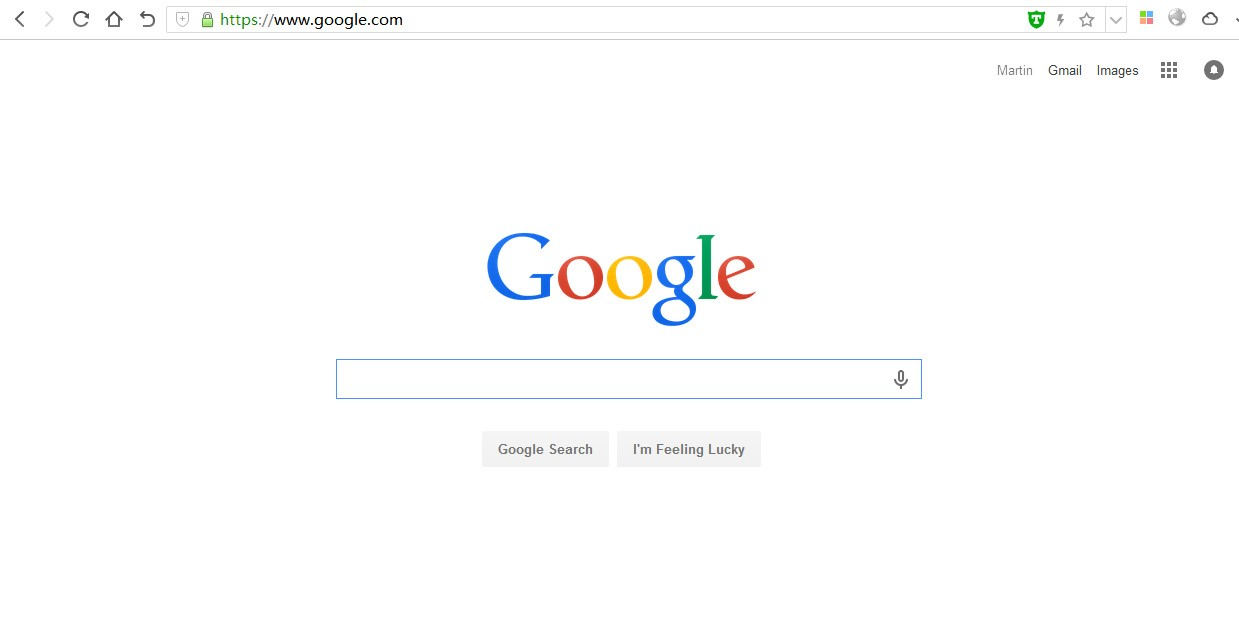
\includegraphics[width=0.97\linewidth]{2.3.2}
        \end{minipage}
        }
        \vspace{-1em}
    \end{figure}
    \vspace{-4em}
    \begin{multicols}{2}
        \begin{enumerate}[label=\Alph*.]
            \item 背景颜色
            \item 第一个网站提供了对结果数量的控制
            \item 第二个网站只包含必要的UI组件
            \item 第二个网站的配色方案更优
        \end{enumerate}
    \end{multicols}
    \vspace{-1em}
\end{problem}



\begin{problem}
	以下关于短时记忆描述正确的是:
	\uline{A}    
    \vspace{-0.8em}
    \begin{multicols}{2}
        \begin{enumerate}[label=\Alph*.]
            \item 短时记忆的容量是有限的
            \item 短时记忆的容量是无限的
            \item 短时记忆的容量为零
            \item 短时记忆的容量很大,但容量有限
        \end{enumerate}
    \end{multicols}
    \vspace{-1em}
\end{problem}



\begin{problem}
	假设需要判断某应用程序的配色方案是否恰当。对于该测试任务,您将使用:
	\uline{B}    
    \vspace{-0.8em}
    \begin{multicols}{2}
        \begin{enumerate}[label=\Alph*.]
            \item  低保真模型
            \item  高保真模型
        \end{enumerate}
    \end{multicols}
    \vspace{-1em}
\end{problem}



\begin{problem}
	原型阶段跟在哪一个开发阶段的后面?
	\uline{C}    
    \vspace{-0.8em}
    \begin{multicols}{4}
        \begin{enumerate}[label=\Alph*.]
            \item 评估
            \item 构建应用程序
            \item 理解用户需要
            \item 以上都不对
        \end{enumerate}
    \end{multicols}
    \vspace{-1em}
\end{problem}



\begin{problem}
	``人物角色不是特定于上下文的,所以它可以很容易地被重复使用”,该表述是
	\uline{B}    
    \vspace{-0.8em}
    \begin{multicols}{2}
        \begin{enumerate}[label=\Alph*.]
            \item 正确的
            \item 错误的
        \end{enumerate}
    \end{multicols}
    \vspace{-1em}
\end{problem}



\begin{problem}
	以用户为中心的设计方法很重要,这是因为:
	\uline{B}    
    \vspace{-0.8em}
    \begin{multicols}{2}
        \begin{enumerate}[label=\Alph*.]
            \item 用户需要被教导如何使用设计产品
            \item 系统设计应该对用户足够直观
            \item 系统设计应特别迎合使用者的需要
            \item 在进行设计时,有必要了解用户所处的环境
        \end{enumerate}
    \end{multicols}
    \vspace{-1em}
\end{problem}



\begin{problem}
	现实世界中对事务的控制及其影响之间的关系指的是:
	\uline{C}    
    \vspace{-0.8em}
    \begin{multicols}{3}
        \begin{enumerate}[label=\Alph*.]
            \item 可见性 Visibility
            \item 功能可见性 Affordance
            \item 映射 Mapping
        \end{enumerate}
    \end{multicols}
    \vspace{-1em}
\end{problem}



\begin{problem}
	GOMS 表示的是:
	\uline{A}    
    \vspace{-0.8em}
    \begin{multicols}{2}
        \begin{enumerate}[label=\Alph*.]
            \item  Goals, operation, methods and selection rules
            \item  Goals, objects, models and selection rules
            \item  Goals, operations, methods and state rules
            \item  Goals, operations, models and state rules
        \end{enumerate}
    \end{multicols}
    \vspace{-1em}
\end{problem}



\begin{problem}
	为探索小孩子们在一起是如何交谈的,并调查一种新型产品是否能帮助他们更积极地参与其中,可使用如下哪种技术:
	\uline{B}    
    \vspace{-0.8em}
    \begin{multicols}{4}
        \begin{enumerate}[label=\Alph*.]
            \item 可用性测试
            \item 实地研究
            \item 预测性评估
            \item DECIDE 框架
        \end{enumerate}
    \end{multicols}
    \vspace{-1em}
\end{problem}



\begin{problem}
	关于启发式评估,以下论证正确的是:
	\uline{A}    
    \begin{enumerate}[label=\Alph*.]
        \item 启发式评估是一种基于专家的评估方法
        \item 专家应用启发式评估时,会从自身使用经验出发对界面进行判断
        \item 启发式评估的结果只有界面中潜在的可用性问题列表
        \item 当界面元素存在多个可用性问题时,只需列举其中一个问题即可
    \end{enumerate}
\end{problem}


	\subsubsection*{二、填空题}
\setcounter{problemname}{0}

\begin{problem}
以Windows和Mac操作系统为代表的界面范式被称作 \myunderline{图形用户界面}。
\end{problem}


\begin{problem}
帮助我们把相继出现的一组图片组合成一个连续的图像序列,产生动态的影像信息的是\myunderline{感觉记忆(瞬时记忆)}。
\end{problem}


\begin{problem}
在EEC模型中,用户为达目标而制定的动作与系统允许的动作之间的差别被称作\myunderline{执行隔阂}。
\end{problem}



\begin{problem}
在简易可用性工程中,建议将\myunderline{边做边说法}和启发式评估结合使用,可以发现大部分软件可用性问题。
\end{problem}



\begin{problem}
对于主流用户很少使用,但自身需要更新的功能,可使用\myunderline{隐藏}策略进行简化。
\end{problem}


	\subsubsection*{\S 简答题}
\setcounter{problemname}{0}

\begin{problem}
写出下列核心词汇的英文全称:
\begin{enumerate}[label=(\arabic*)]
    \item 【2015、2021】人机交互:\myunderline{Human Computer Interaction}
    \item 【2015、2021、2023】以用户为中心的设计:\myunderline{User Centered Design}
    \item 【2015】启发式评估:\myunderline{heuristic evaluation}
    \item 【2015】卡片分类方法:\myunderline{Card Sorting}
    \item 【2015】用户角色:\myunderline{User Role}
    \item 【2014、2015】WIMP:\myunderline{Window、Icon、Menu、Pointer}
    \item 【2014、2023】KLM、GOMS \myunderline{Goal + Operator + Method + Selection}、HTA
    \item 【2022】WYSIWYG:\myunderline{When you see is when you get}
\end{enumerate}
\end{problem}
\vspace{0.25em}


\begin{problem}[2015]
评价观点:“人机交互就是人机界面设计”。
\end{problem}

\begin{solution}
不完全的,人机交互的一部分是人机界面交互,还会涉及到心理学等多个其他学科。
\end{solution}



\begin{problem}[2015、2016]
解释什么是边做边说(think aloud),并分析其在交互评估中的作用。
\end{problem}

\begin{solution}
让真实用户在使用系统执行一组特定任务的时候,说出自己的想法以及想要做的事情。

\vspace{-0.8em}
\begin{multicols}{2}
    \begin{itemize}
        \item 帮助观察人员了解他们的思考过程
        \item 当用户沉默时,观察人员可以提醒用户
        \item 优点:简单、只需要很少的专业技术
        \item 缺点:不自然,可能改变人们执行任务的方式
    \end{itemize}
\end{multicols}
\vspace{-1em}
\end{solution}



\begin{problem}[2015]
有人说“以用户为中心就是什么都听用户的”,试评价此观点并分析。
\end{problem}

\begin{solution}
错误,应当充分利用用户的技能和判断力,而不是完全交由其完成。
\end{solution}



\begin{problem}[2016]
举出一个浏览器预测用户行为的功能实例。
\end{problem}

\begin{solution}
记录下载的位置。对应的设计原则:灵活性和高效性。
\end{solution}



\begin{problem}[2015]
解释什么是启发式评估,并描述其评估过程和优缺点。
\end{problem}

\begin{solution}
启发式评估是非正式可用性检查技术,由可用性专家完成,是一种灵活而又相当廉价的评估方式。

评估过程:
\begin{enumerate}[label=\arabic*.]
    \item 准备:确定可用性准则、组成评估组、计划地点、准备材料、设定评估和记录的策略
    \item 评估:建立对系统概况的感知、发现并列出系统中违背可用性原则之处
    \item 结果分析:回顾问题、建立亲和图、判定每个问题、判断问题的严重性、确定解决问题的建议
    \item 报告汇总:汇总评估组会议结果、形成报告、审查报告
\end{enumerate}

启发式评估的优点:
\begin{itemize}
    \item 不涉及用户,所以面临的实际限制和道德问题较少
    \item 成本相对较低,不需要特殊设备,而且较为快捷
\end{itemize}

启发式评估的缺点:
\begin{itemize}
    \item 评估人员需要经过长时间的训练才能成为专家:理想专家应同时具备交互设计和产品应用域的知识
    \item 可能出现“虚假警报”(“专家每找到一个真实的可用性问题,将发出约一个假警报(1.2),忽略大约半个问题(0.6)”)
\end{itemize}
\end{solution}



\begin{problem}[2015]
举出5个近年来出现的新型人机交互设备并说明其应用。
\end{problem}

\begin{solution}
脑机交互、VR设备、AR设备、智能手表、智能眼镜。
\end{solution}



\begin{problem}[2015、2023]
举出记忆的三种类型,并简述特点。
\end{problem}

\begin{solution}
\begin{enumerate}[label=\arabic*.]
    \item 感觉记忆:又称瞬时记忆,在人脑中持续约为1秒钟
    \vspace{-0.25em}
    \begin{itemize}
        \item 帮助我们把相继出现的一组图片组合成一个连续的图像序列,产生动态的影像信息
    \end{itemize}
    \item 短时记忆:感觉记忆经编码后形成,又称工作记忆,约保持30秒
    \vspace{-0.25em}
    \begin{itemize}
        \item 储存的是当前正在使用的信息,是信息加工系统的核心,可理解为计算
        机的内存
        \item 短时记忆的存储能力约为$7 \pm 2$个信息单元
    \end{itemize}
    \item 长时记忆:短时记忆中的信息经进一步加工后会变为长时记忆
    \vspace{-0.25em}
    \begin{itemize}
        \item 只有与长时记忆区的信息具有某种联系的新信息才能够进入长时记忆
        \item 长时记忆的信息容量几乎是无限的
    \end{itemize}
\end{enumerate}
\end{solution}



\begin{problem}[2015、2016、2021、2023]
运用学过的知识解释什么是心智模型,并说明这对界面设计有何指导意义。
\end{problem}

\begin{solution}
心智模式又叫心智模型。所谓心智模式是指深植我们心中关于我们自己、别人、组织及周围世界每个层面的假设、形象和故事。并深受习惯思维、定势思维、已有知识的局限。

让概念模型和心智模型尽可能贴近。
\end{solution}



\begin{problem}[2015、2016、2021]
有4个相互独立的任务A、B、C、D和8名背景相似测试者,试写出人机交互测试的步骤与人物分配,并简述原因。
\end{problem}

\begin{solution}
将8个人物分为4个小组,每个小组按照不同的顺序执行任务:ABCD、BDAC、DCBA、CADB

原因:消除顺序效应、个体差异的影响。
\end{solution}



\begin{problem}[2012]
在使用微软的软件时,用户可以选择在工具栏图标的下方增加文本标签。请说明为什么点击带有标签的工具更为容易(假设即使没有标签,用户也知道工具的用途)。
\end{problem}

\begin{solution}
加大了图标面积。根据Fitts定律,在其他条件不变的情况下,目标越大,访问越快

改变了工具栏图标过于拥挤的情况
\end{solution}



\begin{problem}[2012]
可用性实验室通常带有单面透光的墙镜。评估人员透过墙镜观察用户执行任务的情况,但用户看不到评估人员。评估人员是否应向用户说明这一点。
\end{problem}

\begin{solution}
需要,有简短的协议书。
\end{solution}



\begin{problem}[2012]
为教学支持系统的评估工作准备一份简短的协议书。
\end{problem}

\begin{solution}
\vspace{-0.8em}
\begin{multicols}{2}
    \begin{enumerate}[label=\arabic*.]
        \item 解释清楚试验的目的
        \item 说明保密事项
        \item 试验相关设备的使用方法
        \item 对测试过程的特殊要求,是否边做边说等
        \item 用户可自由表达对产品的意见
        \item 告诉参加者试验过程中需要进行笔录、录音和录像的目的
        \item 欢迎用户提问
        \item 用户有随时终止测试的权利 
        \item 对用户话语的使用征得同意,并选择匿名方式
    \end{enumerate}
\end{multicols}
\vspace{-1em}
\end{solution}



\begin{problem}[2013]
列举6种界面设计人员可用于管理用户注意力的方式。
\end{problem}

\begin{solution}
\vspace{-0.8em}
\begin{multicols}{2}
    \begin{enumerate}[label=\arabic*.]
        \item 使用大的屏幕元素,是屏幕元素占据更多的屏幕空间
        \item 使用更少的组件,尽量减少不必要的组件出现在界面上
        \item 注意反馈系统状态或活动进度
        \item 使用鲜明的色彩
        \item 使用适当的对话框
        \item 使用合适的方法,课根据格式塔原理进行设计
    \end{enumerate}
\end{multicols}
\vspace{-1em}
\end{solution}



\begin{problem}[2012、2013]
请分别使用一句话解释GOMS模型四个字母所代表的含义,以及为什么使用GOMS分析未必能预测出最好的设计。
\end{problem}

\begin{solution}
GOMS是关于人类如何执行认知-动作型任务以及如何与系统交互的理论模型。
\begin{itemize}
    \item Goal-目标:用户要达到什么目的。
    \item Operator-操作:任务执行的底层行为,不能分解,为达到目标而使用的认知过程和物理行为。如点击鼠标。
    \item Method-方法:如何完成目标的过程,即对应目标的子目标序列和所需操作。如移动鼠标,输入关键字,点击Go按钮。
    \item Selection-选择规则:确定当有多种方法时选择和方法。GOMS认为方法的选择不是随机的。
\end{itemize}

局限性:
\vspace{-0.8em}
\begin{multicols}{2}
    \begin{enumerate}[label=\arabic*.]
        \item 假设用户完全按一种正确的方式进行人机交互,没有清楚地描述错误处理的过程
        \item 只针对那些不犯任何错误的专家用户
        \item 任务之间的关系描述过于简单
        \item 忽略了用户间的个体差异
    \end{enumerate}
\end{multicols}
\vspace{-1em}
\end{solution}



\begin{problem}[2013]
简述执行隔阂与评估隔阂的概念,并说明它们对交互设计有何指导意义。
\end{problem}

\begin{solution}
执行隔阂:用户为执行达到的目标而设定的活动与系统允许的活动不符。

评估隔阂:系统状态与用户设想的想象有差距。

指导意义:
\begin{itemize}
    \item 系统活动的有效性,即由执行隔阂评估得到。设计师的目标就是使系统的设计与用户活动的期望相符合,这样才是最好的设计。
    \item 对系统状态的评估越简单,评估隔阂就越小。这说明在设计时应充分考虑即使将系统的状态,活动进度,用户当前的位置的信息反馈给用户。
\end{itemize}
\end{solution}



\begin{problem}[2013、2023]
在开展用户测试时,用户数量的选取通常在什么范围,并简要说明为什么在该范围是比较恰当的。

在开展用户测试时,Jacob Nielsen对于用户数量的选取有何建议?并简要阐述为什么该范围是比较恰当的?以及应用该数量进行实验的时候有何注意事项。
\end{problem}

\begin{solution}
$5 \sim 12$人。

因为根据统计可知,测试用户数量越多,发现的可用性问题及用户体验问题越多。当用户人数达到15人时,基本可以发现98\%的可用性问题。但出于成本和效率的考虑,$5 \sim 12$个用户测试人数是比较合理的。

了解用户的特性有助于选择典型用户:要尽可能接近实际用户;通常也需要平衡性别比例。
\end{solution}



\begin{problem}[2013]
“以用户为中心”是交互设计领域的主要思想,其含义是产品设计要充分满足用户期望,并确实取得了很多成功。你认为这种思想可能存在的局限性是什么,试举出现实生活中没有根据该思想但确实取得成功的产品。
\end{problem}

\begin{solution}
“以用户为中心”的设计(UCD)在理论上几乎达到完美,但是经过长期的设计实践,人们发现这种思想仍存在局限性:
\vspace{-0.8em}
\begin{multicols}{2}
    \begin{enumerate}[label=\arabic*.]
        \item 影响产品的创新性
        \item 可操作性受到时间、预算和任务规模的限制
        \item 忽视了人的主观能动性和对技术的适应能力
    \end{enumerate}
\end{multicols}
\vspace{-1em}
\end{solution}



\begin{problem}[2013]
解释击键层次模型并描述其用途。
\end{problem}

\begin{solution}
击键层次模型是1983年由Card等人提出的,是对用户执行情况进行量化预测,仅涉及任务性能的一个方面:时间。

用途:
\vspace{-0.8em}
\begin{multicols}{2}
    \begin{enumerate}[label=\arabic*.]
        \item 预测无错误情况下专家用户在下列输入前提下完成任务的时间
        \item 便于比较不同系统
        \item 确定何种方案能最有效地支持特定任务
    \end{enumerate}
\end{multicols}
\vspace{-1em}

使用:执行时间预测方法
\vspace{-0.8em}
\begin{multicols}{2}
    \begin{enumerate}[label=\arabic*.]
        \item 列出操作次序,累加每一项操作的预计时间
        \item $T_{execute} = T_k + T_P + T_h + T_d + T_m + T_r$
    \end{enumerate}
\end{multicols}
\vspace{-1em}
\end{solution}



\begin{problem}[2021]
若要将英文句子``I do like using the keystroke level model.",中的``like"替换为``hate",使之变为``I do hate using the keystroke level model."假设当前用户的手放在键盘上,且通过简单的删除和插入操作完成替换动作,应用击键层次模型对新手打字员执行该交互任务的时间进行预测。(各操作的时间见下表)
\begin{figure}[H]
    \vspace{-0.5em}
    \centering
    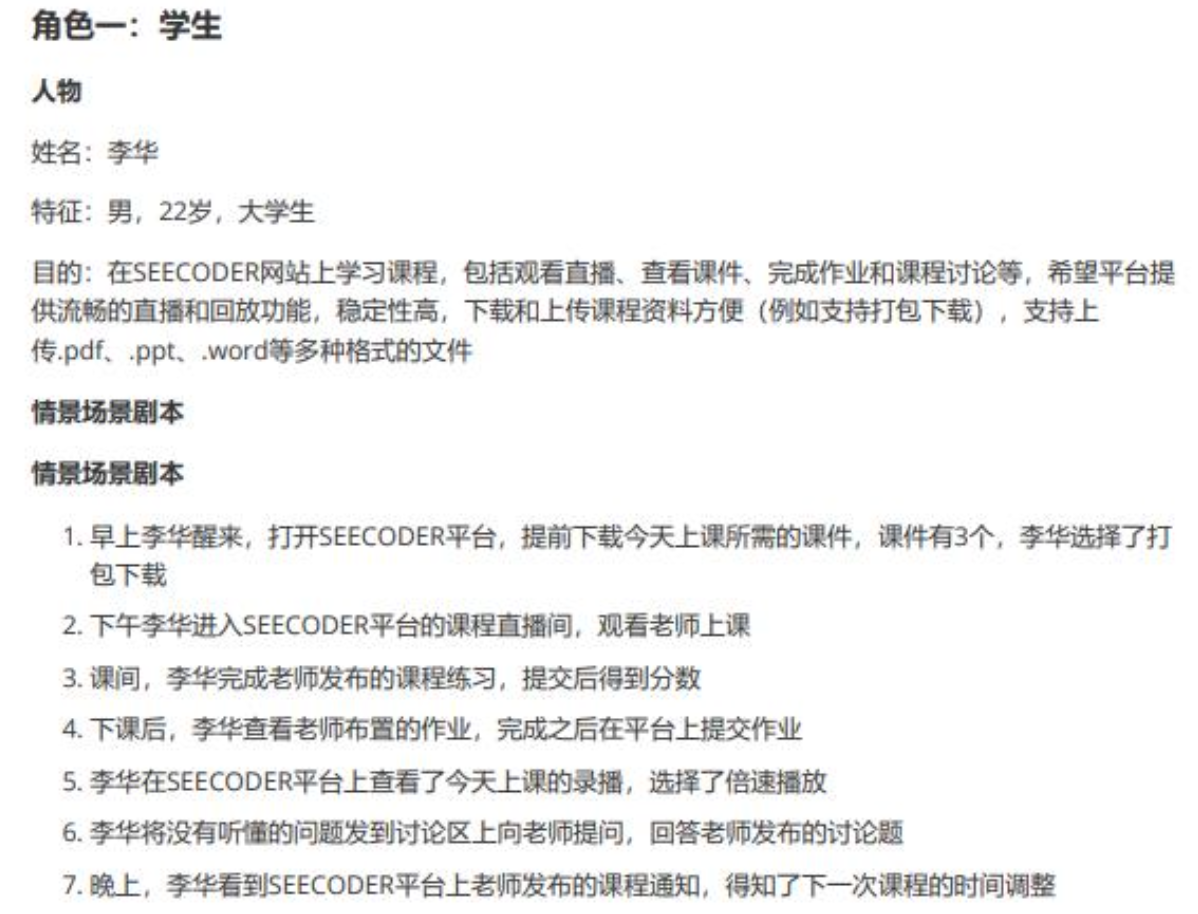
\includegraphics[width=0.7\textwidth]{2.png}
    \vspace{-1em}
\end{figure}
\end{problem}
    
\begin{solution}
操作序列:$M$(任务准备)、$H$(将手放在鼠标上)、$P$(将鼠标移到单词)、$P_1$(选择单词)、$H$(回到键盘)、$M$(准备键入)、$8K$(键入8下)
    
$T_{execute} =2\times M+ 2\times H + P +P_1 + 8\times K=7.04 (K=0.28)$
\end{solution}


\begin{problem}[2013]
请给出如下使用文字描述的层次化分析所对应的图形描述。
\end{problem}

\begin{solution}

\begin{wraptable}{r}{0.73\textwidth}
    \centering
    \vspace{-1.5em}
    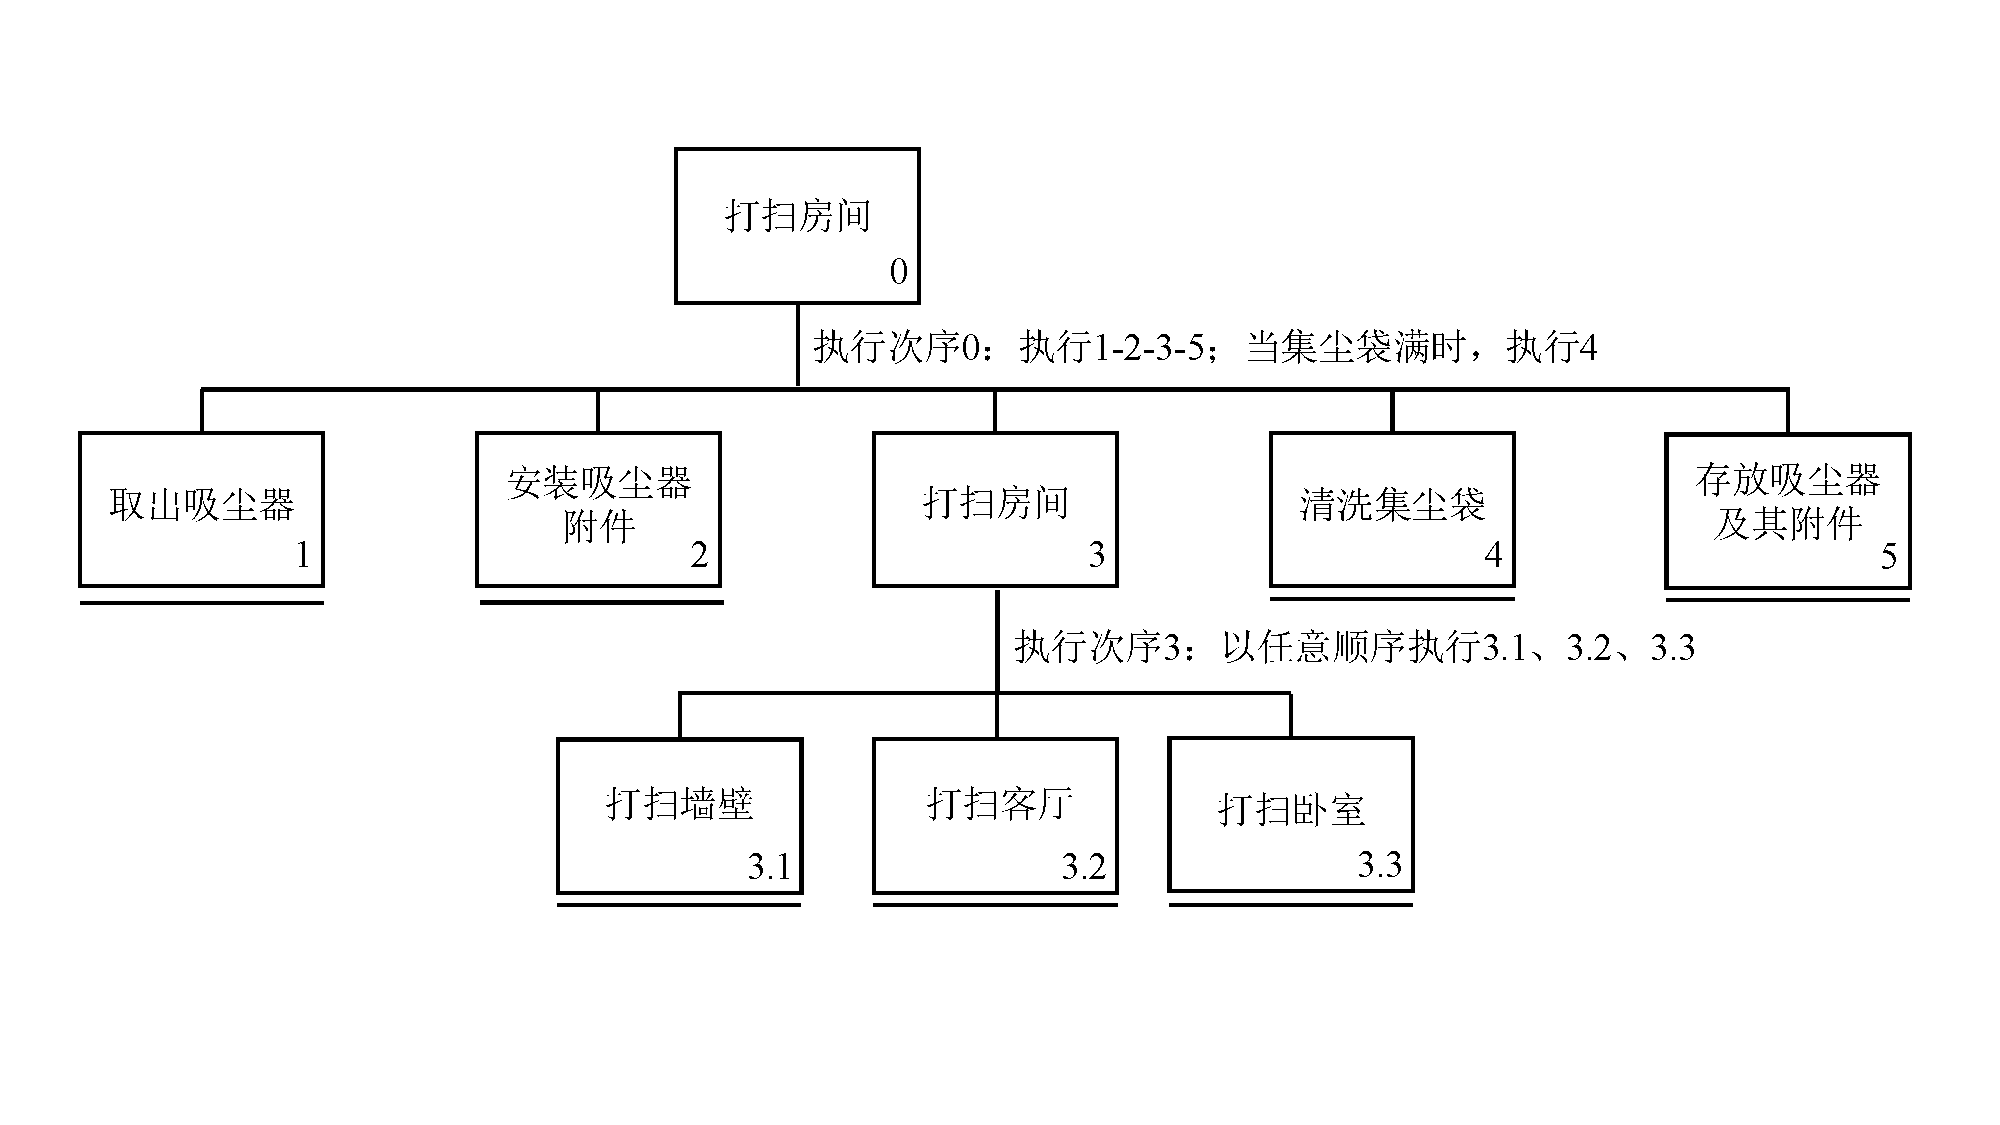
\includegraphics[width=0.73\textwidth]{21.pdf}
    \vspace{-3.5em}
\end{wraptable}
{\songti 0. 打扫房间
\vspace{-0.2em}
\begin{enumerate}[label=\arabic*.]
    \item 取出吸尘器
    \item 安装吸尘器附件
    \item 打扫房间
    \vspace{-0.3em}
    \begin{enumerate}[label=3.\arabic*.]
        \item 打扫墙壁
        \item 打扫客厅
        \item 打扫卧室
    \end{enumerate}
    \item 清洗集尘袋
    \item 存放吸尘器及其附件
\end{enumerate}
执行次序0:顺序执行1、2、3、5;当集尘袋满时,执行4

执行次序3:以任意顺序执行3.1、3.2、3.3}
\end{solution}



\begin{problem}[2021]
随着电子商务发展越来越成熟,网上购物已经成为人们生活中的一部分,不管是衣服还是电器或者日常生活用品,选择在网上购物的人逐渐增多。请分析用户的在线购物行为,并给出该过程的层次化任务分析的文字描述和图形表示。
\end{problem}

\begin{solution}
\vspace{-0.8em}
\begin{multicols}{2}
    \begin{enumerate}[label=\arabic*.,start=0]
        \item 在线购物
        \vspace{-0.3em}
        \begin{enumerate}[label=\arabic*.]
            \item 打开在线购物软件
            \item 检索想要购买的物品
            \begin{enumerate}[label=2.\arabic*]
                \item 使用在线购物软件搜索栏
                \item 输入购买的物品的名称和特征
                \item 找出需要购买的物品
            \end{enumerate}
            \item 点开想要购买的物品的详情页面
            \item 支付并购买该物品
        \end{enumerate}
    \end{enumerate}
\end{multicols}
\vspace{-1em}

执行次序0:执行1-3-4:如果首页没有想要购买的产物品,则执行次序2-3-4
\end{solution}



\begin{problem}[2022]
作为组织者组织一次会议是一项非常繁琐的工作,涉及到很多细节事务。在用户体验设计中,层次化任务分析用来分析并描述用户如何为达到目标所进行的一系列任务,以及用户与软件系统是如何交互的。如果你将\textbf{组织一次会议},请使用层次化任务分析技术完成会议组织的层次化任务分析的文字和图形描述。
\end{problem}

\begin{solution}
\begin{figure}[H]
    \vspace{-0.5em}
	\centering
	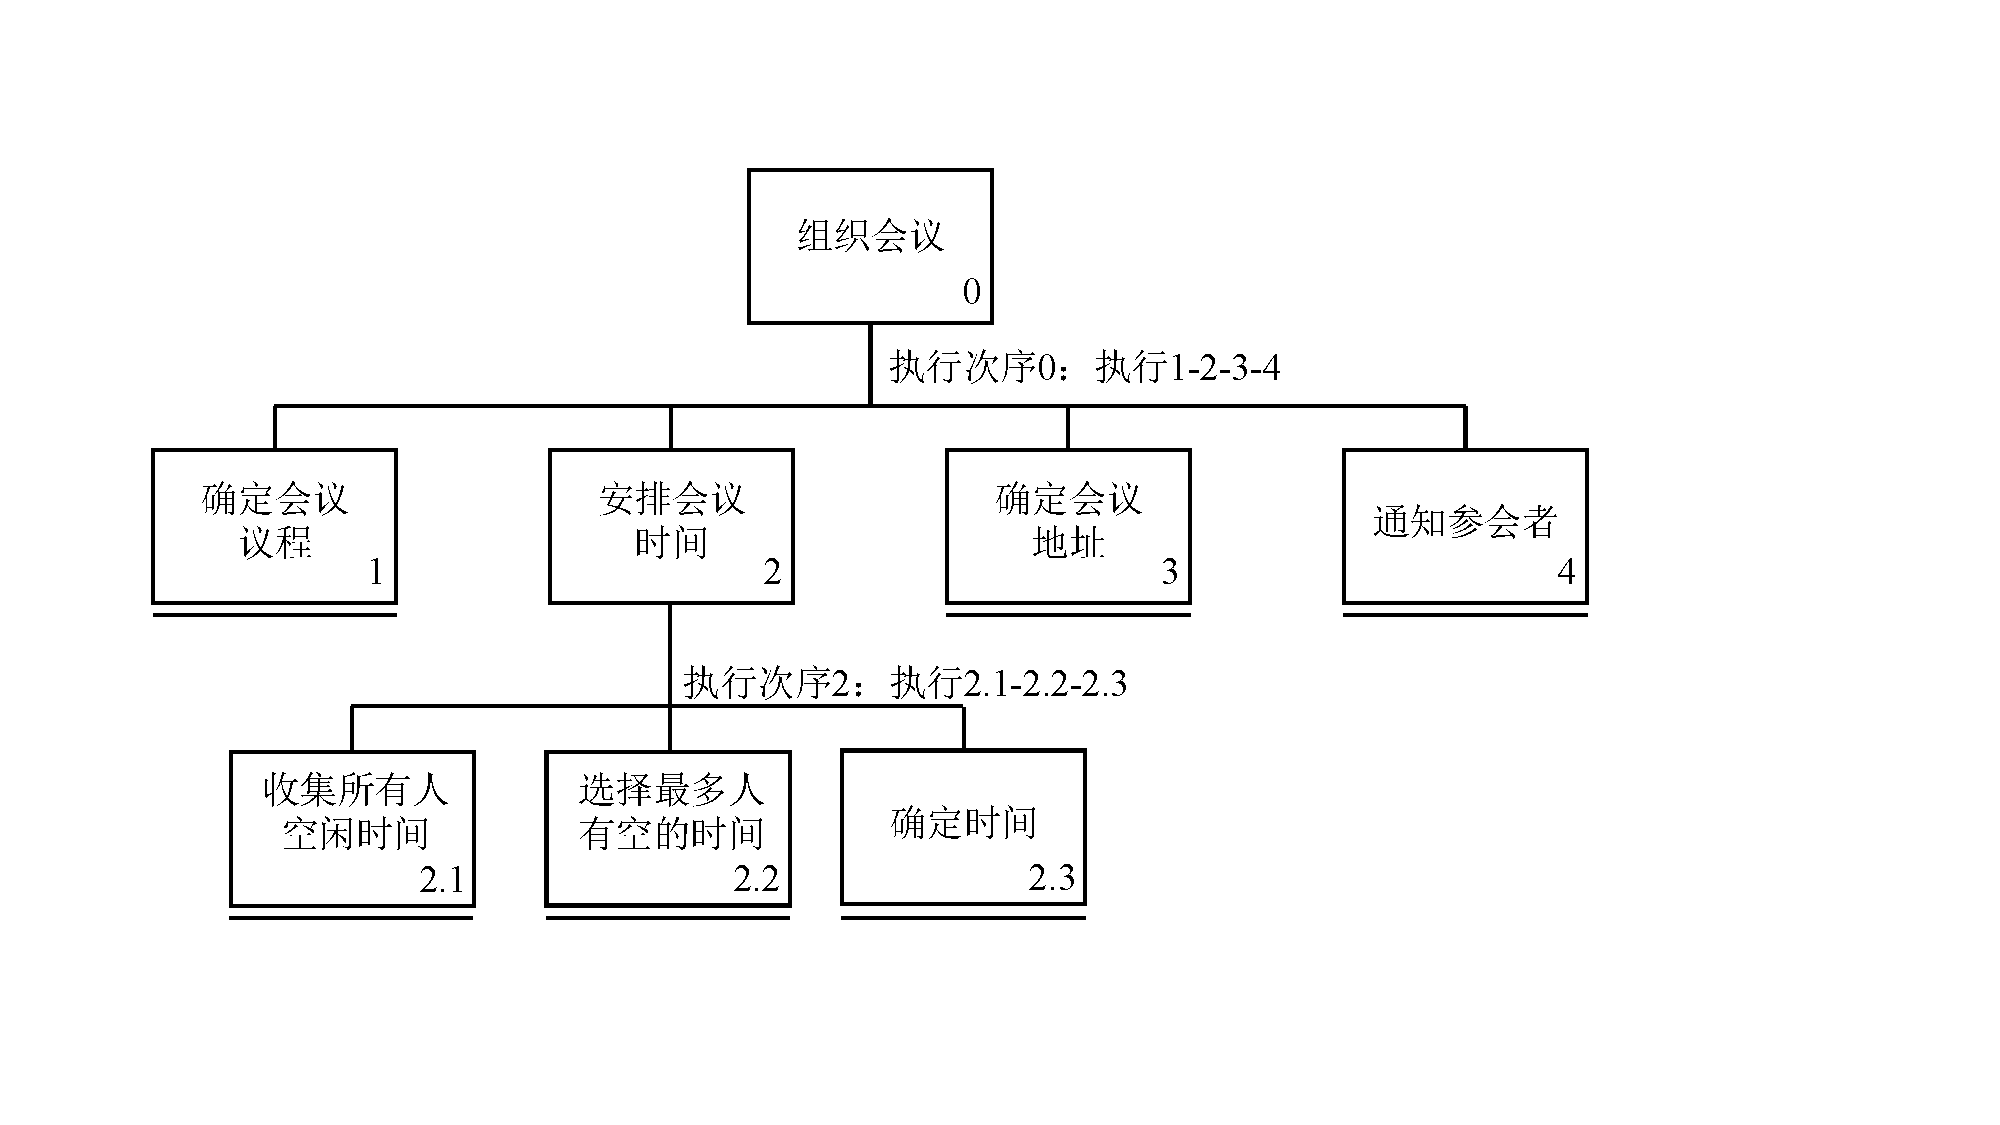
\includegraphics[width=0.7\textwidth]{3.pdf}
    \vspace{-1em}
\end{figure}
\end{solution}



\begin{problem}[2016]
现在处于怎样的人机交互时代?WIMP四个字母的含义是什么?
\end{problem}

\begin{solution}
图形用户界面GUI时期(Graphical User Interface);WIMP:Windows, Icon, Menu, Pointer
\end{solution}



\begin{problem}[2016、2021]
课程中曾以视频形式向大家介绍了“第六感系统”,简述该系统并分析它相较今天的主流交互形式有哪些区别和特点?
\end{problem}

\begin{solution}
硬件组成:这套名为“第六感”的设备,由一个网络摄像头、一个微型投影仪附加镜子、一个挂在脖子上的电池包和一台可以上网的3G手机组成。

核心功能模块:将眼前的现实世界变成电脑屏幕,为自己提供数字服务。\footnote{\url{https://lcx.cc/post/1550/}}
\end{solution}



\begin{problem}[2016]
根据操作计算机水平差异对用户进行分类并说明各自特点以及针对性的交互设计。
\end{problem}

\begin{solution}
\vspace{-0.5em}
\begin{table}[H]
\centering
\resizebox{\textwidth}{!}{\begin{tabular}{|c|c|c|}
\hline
\textbf{用户分类} & \textbf{特点} & \textbf{针对交互设计} \\ \hline
新手用户 & 敏感,开始容易有挫败感 & 解释的菜单项等 \\ \hline
中间用户 & 需要工具,指导如何使用参考资料、高级功能的使用让其放心 & 工具提示,在线帮助,高级特性 \\ \hline
专家用户 & 欣赏更新且强大的功能,不会受复杂度的影响 & 快捷键 \\ \hline
\end{tabular}}
\end{table}
\vspace{-1em}
\end{solution}



\begin{problem}[2014、2016、2023]
面对对话框内容的拥挤,简述三种管理的策略。(简化设计的策略有哪些?分别适用什么场合?)

对界面上不是很重要的组件和信息,为避免其分散用户的注意力可以采用哪种简化设计策略?({\kaishu 隐藏})
\end{problem}

\begin{solution}
\begin{enumerate}[label=\arabic*.]
    \item 删除:删除杂乱的特性,关注核心,砍掉残缺功能:删除错误;删除视觉混乱(减少用户必须处理的信息,集中注意力在真正重要的内容上);删减文字(删除不必要内容可以让读者对自己看到的内容更有自信);精简句子(让文字变得更加简洁、清晰、有说服力)
    \item 组织:分块;确定清晰的分类标准;利用不可见的网格来对齐界面元素,重要的元素要大一些,不太重要的界面元素应该小一些;把相似元素放在一起
    \item 隐藏:主流用户很少使用,但自身需要更新的功能;事关细节(对服务器进行配置或设计邮件签名);选项和偏好(修改绘图应用的单位);特定于地区的信息(如时间和日期需频繁自动更新的信息)
    \item 转移:有时候,把某项任务的某些内容(如输入信息)转移到不同的平台(移动平台/桌面平台)上可能是一种更好的选择;让用户做擅长的事情
\end{enumerate}
\end{solution}



\begin{problem}[2016]
被作为“计算机内存”是哪一阶段的记忆?有什么特点?对HCI的要求是什么?
\end{problem}

\begin{solution}
短时记忆,是感觉记忆经过编码得到的,能持续30s,存储了正在使用的信息。

使用$7 \pm 2$原则进行交互设计。
\end{solution}



\begin{problem}[2012、2014]
如何确保问卷中的问题对于用户而言是重要且完备的?
\end{problem}

\begin{solution}
问卷设计原则:
\vspace{-0.8em}
\begin{multicols}{2}
    \begin{enumerate}[label=\arabic*.]
        \item 应确保问题明确,具体
        \item 在可能时,采用封闭式问题并提供充分的答案选项
        \item 对于征求用户意见的问题,应提供一个“无看法”的答案选项
        \item 注意提问次序,先提出一般化问题,再提出具体问题
        \item 避免使用复杂的多重问题
        \item 在使用等级标度时,应设定适当的等级范围,并确保它们不重叠
        \item 避免使用术语
        \item 明确说明如何完成问卷
        \item 在设计问卷时,既要做到紧凑,也应适当留空
    \end{enumerate}
\end{multicols}
\vspace{-1em}
\end{solution}



\begin{problem}[2014]
对于“简单就是美”发表看法。
\end{problem}

\begin{solution}
“简单就是美”在人机交互领域中绝对是个重要的原则。简洁的界面和操作流程能够提高用户体验,降低学习曲线,使用户更轻松地完成任务。当设计变得复杂时,用户可能感到困惑,甚至放弃使用。简单的设计也有助于提高可用性,因为用户更容易理解和记忆界面的各个元素。

但是,简单并不意味着缺乏功能或深度。好的设计应该在保持简单的同时,满足用户的需求,并提供足够的功能和灵活性。简单之美在于精心的设计和合理的功能布局,而不是简单到极端而忽略了用户的真实需求。
\end{solution}



\begin{problem}[2022]
Mark Weiser 在 ``The computer for the 21st century" 一文中提到要让计算机消失在背景中,请概述你对这句话的理解。\textit{A new way of thinking about computers, one that takes into account the human world and allows the computers themselves to vanish into the background.}
\end{problem}

\begin{solution}
技术应该是不显眼的、直观的和易于使用的。
\end{solution}



\begin{problem}[2014、2021]
大作业中人机交互的改善。

简述一条在他人项目进行启发式评估的作业中发现的一个可用性问题,请简要描述该问题以及其违反的启发式规则。
\end{problem}



\begin{problem}[2021、2023]
请简述为什么图形用户界面可以摒弃$7 \pm 2$的设计约束,在界面上放置多个界面组件?
\end{problem}

\begin{solution}
因为图形用户界面不是基于记忆的,而是基于认知和识别的。

图形用户界面(GUI)相对于命令行界面(CLI)的一个显著优势是其能够放置和管理大量的界面组件,而不受 $7 \pm 2$ 的设计约束。这个数字 $7 \pm 2$ 是由心理学家乔治·米勒提出的米勒定律,指的是人们在短时记忆中能够有效处理的信息单元数量。然而,在GUI中,我们能够摆脱这个限制的原因有几点:

\begin{enumerate}[label=\arabic*.]
    \item \textbf{可视化表示:} GUI通过图形元素的可视化表示,使用户更容易理解和识别界面上的元素。图标、按钮、菜单等图形元素能够通过形状、颜色和位置等特征传达信息,减轻了用户在界面上寻找和理解元素的认知负担。
    \item \textbf{多窗口和分层设计:} GUI允许使用多窗口和分层设计,使用户能够在界面上同时处理多个任务。每个窗口或层次结构中的组件可以独立存在,用户可以方便地切换、最小化或关闭这些窗口。
    \item \textbf{滚动和搜索功能:} GUI提供了滚动和搜索功能,使用户能够查看和访问大量的内容,而不受到屏幕空间的限制。这允许用户在大规模数据集中快速浏览和定位目标。
    \item \textbf{上下文切换:} GUI允许用户通过不同的视图、标签页或面板切换上下文,使得用户能够更有效地组织和管理信息。
\end{enumerate}
\end{solution}



\begin{problem}[2021]
简要描述什么是人物角色,以及在其构建时需要注意什么问题?
\end{problem}

\begin{solution}
人物角色是基于观察到的那些真实人的行为和动机,并且在整个设计过程中代表真实的人;是在人口统计学调查收集到的实际用户的行为数据的基础上形成的综合原型。

要注意那些与软件用户界面设计有关的角色特征;要关注使角色之间彼此相区别的特征;要留心焦点角色 (最常见、最典型的角色)。
\end{solution}



\begin{problem}[2021]
原型是一种用户乐于接受的需求验证方式,请简要描述一下不同类型的原型在使用时的优缺点。
\end{problem}

\begin{solution}
低保真原型简单、便宜、易于修改,但是和最终产品有一定差距。

高保真原型和最终产品较为接近,但是制作时间长,难以修改,并且容易让用户误以为已经有具体的实现。
\end{solution}



\begin{problem}[2021、2022、2023]
请说明Fitts' Law对交互设计有什么启发?

请简述Fitts定律,并应用Fitts定律分析比较饼型菜单(Pie Menu)与普通下拉菜单的交互效率。
\end{problem}

\begin{solution}
\begin{enumerate}[label=\arabic*.]
    \item 大目标、小距离具有优势
    \vspace{-0.4em}
    \begin{itemize}
        \item 对选择任务而言,其移动时间随到目标距离的增加而增加,随目标的大小减小而增加
    \end{itemize}
    \item 屏幕元素应该尽可能多的占据屏幕空间
    \item 最好的像素是光标所处的像素
    \item 屏幕元素应尽可能利用屏幕边缘的优势
    \item 大菜单,如饼型菜单,比其他类型的菜单使用简单
\end{enumerate}

饼形菜单交普通下拉菜单,选项目标更为明显,相关选项并列距离更小,这些都使得饼形菜单的交互效率更高
\end{solution}



\begin{problem}[2021、2023]
在采用观察法进行用户调研时,什么时候可以停止观察?
\end{problem}

\begin{solution}
观察到用户完成任务并确认;用户选择停止任务。
\end{solution}




\begin{problem}[2021、2023]
某设计团队对某个设计问题方案争执不休,最终由公司管理层出面确定了最终方案,请分析他们的做法是否正确,如果不正确请给出你的建议。
\end{problem}

\begin{solution}
不正确,设计问题方案如果出现争执和不确定,应当通过相应的评估手段来解决。
\end{solution}



\begin{problem}[2021、2023]
某人计划针对其设计的产品开展评估实验,他根据DECIDE框架设计了实验的各个步骤,然后就开始招募用户进行实验,请简要分析一下他的做法是否正确?
\end{problem}

\begin{solution}
不正确,需要先进行小规模的预实验。
\end{solution}



\begin{problem}[2022]
“元宇宙”是2022年科技界非常火爆的一个概念。你对元宇宙有什么了解吗?请简要描述一下你眼中的元宇宙,以及元宇宙中可能涉及到的三种关键技术,和它们各自承担的作用。
\end{problem}

\begin{solution}
元宇宙是一个使用尖端技术创造无边界创新体验的概念。它包括虚拟现实、芯片、网络通信、人工智能和区块链。虚拟现实让人们体验不同的虚拟世界,芯片优化数字流程,网络通信连接用户,人工智能优化用户体验,区块链确保数字内容的安全和保护。
\end{solution}



\begin{problem}[2022]
请简要分析一下图形用户界面取代命令行界面得以广泛流行的主要原因是什么?
\end{problem}

\begin{solution}
GUI 比命令行界面更直观、更具视觉吸引力,并且旨在通过将信息置于特定上下文中,以减少信息单元的数量来最大限度地减少用户记忆。

图形用户界面的优点:
\begin{enumerate}[label=\arabic*.]
    \item 图形用户界面可以直接操纵;
    \item 用户可以在窗口内选取任意交互位置,且不同窗口之间可以叠加;
    \item 鼠标;
    \item 图形界面优于字符界面;(不同的交互方式本身在可用性方面并没有根本性的不同,更重要的是更认真对待界面设计的态度)
\end{enumerate}
\end{solution}



\begin{problem}[2022]
在开展某个项目时,某开发人员参考自己的使用习惯对产品的交互设计进行了分析和设计,请分析一下这样做可能存在的问题,以及正确的做法应该如何?
\end{problem}

\begin{solution}
自参考设计:开发人员和实际用户的心智模型可能不同,导致最终产品可能不好用;(局限)

正确做法:充分调研用户,理解你的用户
\end{solution}



\begin{problem}[2022]
微信作为今天生活中十分重要的社交工具,其设计中有很多体现“以用户为中心”的设计细节。请列举2个能够体现为用户设计的案例,并进行简要分析。
\end{problem}

\begin{solution}
用户友好的界面、直观的导航和个性化的内容,使访问和享受更容易。

以用户为中心:
\begin{itemize}
    \item 以真实用户和用户目标作为产品开发的驱动力,而不仅仅是以技术为驱动力
    \item 应能充分利用人们的技能和判断力,应支持用户,而不是限制用户
    \item 需要透彻了解用户及用户的任务,并使用这些信息指导设计
    \item 这是一种设计思想,而不是纯粹的技术
\end{itemize}

以用户为中心的设计原则:
\begin{itemize}
    \item 及早以用户为中心:在设计过程的早期就致力于了解用户的需要
    \item 综合设计:设计的所有方面应当齐头并进地发展
    \item 及早并持续性地进行测试:若实际用户认为设计是可行的,它就是可行的
    \item 迭代设计:大问题往往会掩盖小问题的存在
\end{itemize}
\end{solution}




\begin{problem}[2023]
请简述一条在实践项目中应用课程所学进行交互设计的具体案例,并简要描述所使用的设计方法。
\end{problem}




\begin{problem}[2023]
虚拟现实技术被认为是一把双刃剑。虽然有人觉得它在教育等应用中很吸引人、很实用,但也有一部分人认为它的普及会给社会带来一定的风险。请对此问题进行简要讨论。
\end{problem}

\begin{solution}
虚拟现实(VR)技术确实是一把双刃剑。在教育领域,它能够提供沉浸式学习体验,使学生能够更直观地理解抽象概念,加强记忆和理解。此外,VR还可用于模拟培训,提高实际操作技能,如医学手术或飞行模拟。

然而,随着VR技术的普及,社会面临一些潜在的风险。首先是沉迷问题,一些人可能过度沉浸于虚拟世界,影响现实生活和社交关系。此外,隐私问题也是一个关切点,特别是在虚拟环境中收集和分享个人数据的情况下。可能会出现滥用个人信息的风险。
    
另外,技术的不平等应用也是一个问题。如果虚拟现实教育工具只在一些富裕学校或地区得到推广,而其他地方没有这样的机会,可能会加剧社会中的不平等现象。
    
综合来看,虚拟现实技术的发展需要平衡技术应用的创新与对潜在风险的警惕,以确保其在社会中的良好应用。
\end{solution}



\begin{problem}[2023]
对应“系统设计应遵循特定平台的惯例并接受标准”,且是最容易被违反的启发式设计原则是?{\kaishu \myunderline{一致性和标准化}}
\end{problem}



\begin{problem}[2023]
被称为“最有价值的单个可用性工程方法”的是?{\kaishu \myunderline{边做边说法}}
\end{problem}



\begin{problem}[2023]
四种常用的评估类型分别是什么?
\end{problem}

\begin{solution}
四种评估范型:快速评估、可用性测试、实地研究、预测性评估。
\vspace{-0.5em}
\begin{spacing}{1.2}
    \centering
    \begin{longtable}{|m{2cm}<{\centering}|m{2.9cm}|m{2.9cm}|m{2.9cm}|m{3cm}|}
        \hline
        \textbf{评估范型} & \multicolumn{1}{c|}{\textbf{快速评估}} & \multicolumn{1}{c|}{\textbf{可用性测试}} & \multicolumn{1}{c|}{\textbf{实地研究}} & \multicolumn{1}{c|}{\textbf{预测性研究}} \\ \hline
        用户角色 & 自然行为 & 执行测试任务集 & 自然行为 & 用户通常不参与 \\ \hline
        控制权 & 评估人员实施最低限度控制 & 评估人员密切控制 & 评估人员与用户合作 & 评估人员为专家 \\ \hline
        评估地点 & 自然工作环境或实验室 & 实验室 & 自然工作环境 & 类似实验室的环境,通常在客户处进行 \\ \hline
        适用情形 & 快速了解设计反馈。可使用其他交互范型的技术,如专家评测 & 测试原型或产品 & 常用于设计初期,以检查设计是否满足用户需要,发现问题,发掘应用契机 & 专家(通常是开发顾问)检查原型,可在任何阶段进行。使用模型评测潜在设计的特定方面 \\ \hline
        数据类型 & 通常是定性的非正式描述 & 量化数据,有时是统计数据。可采用问卷调查或访谈搜集用户意见 & 应用草图、场景、例证等的定性描述 & 专家们列出问题清单,由模型导出量化数据,如两种设计的任务执行时间 \\ \hline
        反馈到设计 & 通过草图、例证、报告 & 通过性能评测、错误统计报告等为未来版本提供设计标准 & 通过描述性的例证、草图、场景和工作日志 & 专家列出一组问题,通常附带解决方案建议。为设计人员提供根据模型计算出的时间值 \\ \hline
        基本思想 & 以用户为中心,非常实用 & 基于试验的实用方法,即可用性工程 & 可以是客观观察或现场研究 & 专家检查以实用的启发式原则和实践经验为基础,采用基于理论的分析模型\\ \hline
    \end{longtable}
	\end{spacing}
\vspace{-1em}
\end{solution}
	\subsubsection*{四、设计题}
\setcounter{problemname}{0}

\begin{problem}
指出下面的对话框设计中存在的问题,并给出改进建议。
\begin{figure}[H]
    \vspace{-0.5em}
	\centering
	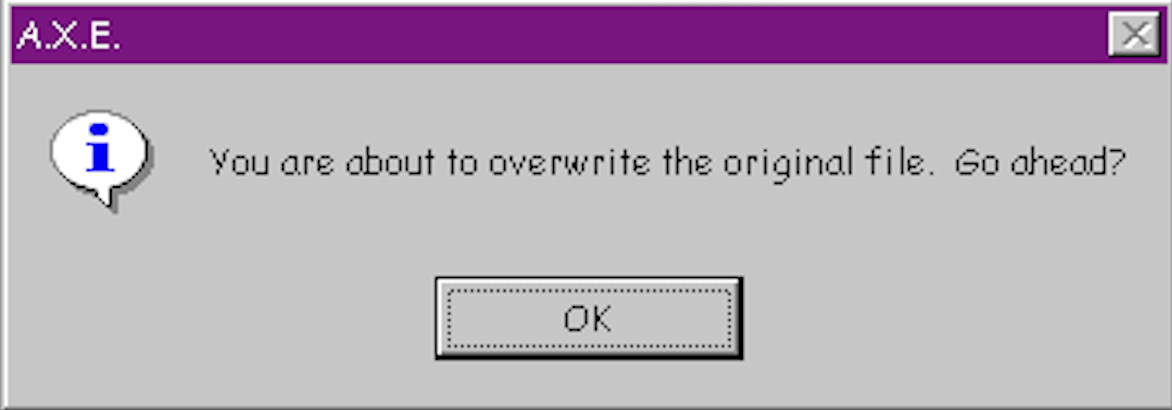
\includegraphics[width=0.5\textwidth]{1.png}
    \vspace{-1em}
\end{figure}
\end{problem}

\begin{solution}
没有讲overwrite的后果;标题A.X.E.是什么意思;只有OK,没有退出机制;
\end{solution}



\begin{problem}
人物角色是交互设计中非常重要的一项技术,能够帮助设计团队做很多设计决策。如下是某团队为某项目构造的人物角色的例子,请分析其中存在的问题,并说明什么是人物角色,以及在构建人物角色时需要注意哪些问题。
\begin{figure}[H]
    \vspace{-0.5em}
	\centering
	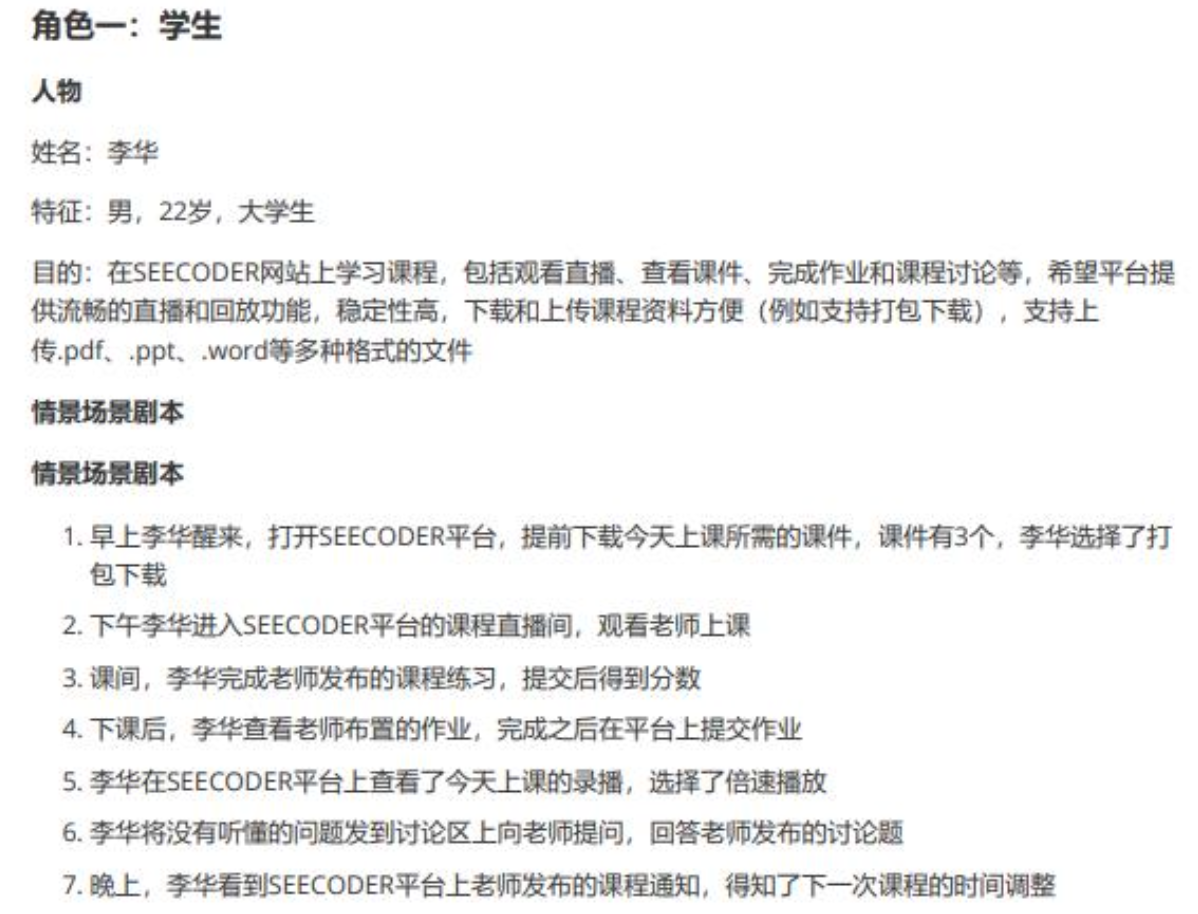
\includegraphics[width=0.7\textwidth]{2.png}
    \vspace{-1em}
\end{figure}
\end{problem}

\begin{solution}
问题:
\begin{enumerate}[label=\arabic*.]
    \item 人物信息构造不完整(没有照片);
    \item 目标不对,目标不是功能(帮助他更好的完成课程学习);
    \item 场景剧本有问题(不能写成使用手册,应该描述需求,不要使用术语,要使用自然语言);
\end{enumerate}

人物角色是基于观察到的那些真实人的行为和动机,并且在整个设计过程中代表真实的人;是在人口统计学调查收集到的实际用户的行为数据的基础上形成的综合原型。

要注意那些与软件用户界面设计有关的角色特征;要关注使角色之间彼此相区别的特征;要留心焦点角色 (最常见、最典型的角色)。
\end{solution}



\begin{problem}
作为组织者组织一次会议是一项非常繁琐的工作,涉及到很多细节事务。在用户体验设计中,层次化任务分析用来分析并描述用户如何为达到目标所进行的一系列任务,以及用户与软件系统是如何交互的。如果你将\textbf{组织一次会议},请使用层次化任务分析技术完成会议组织的层次化任务分析的文字和图形描述。
\end{problem}

\begin{solution}
\begin{figure}[H]
    \vspace{-0.5em}
	\centering
	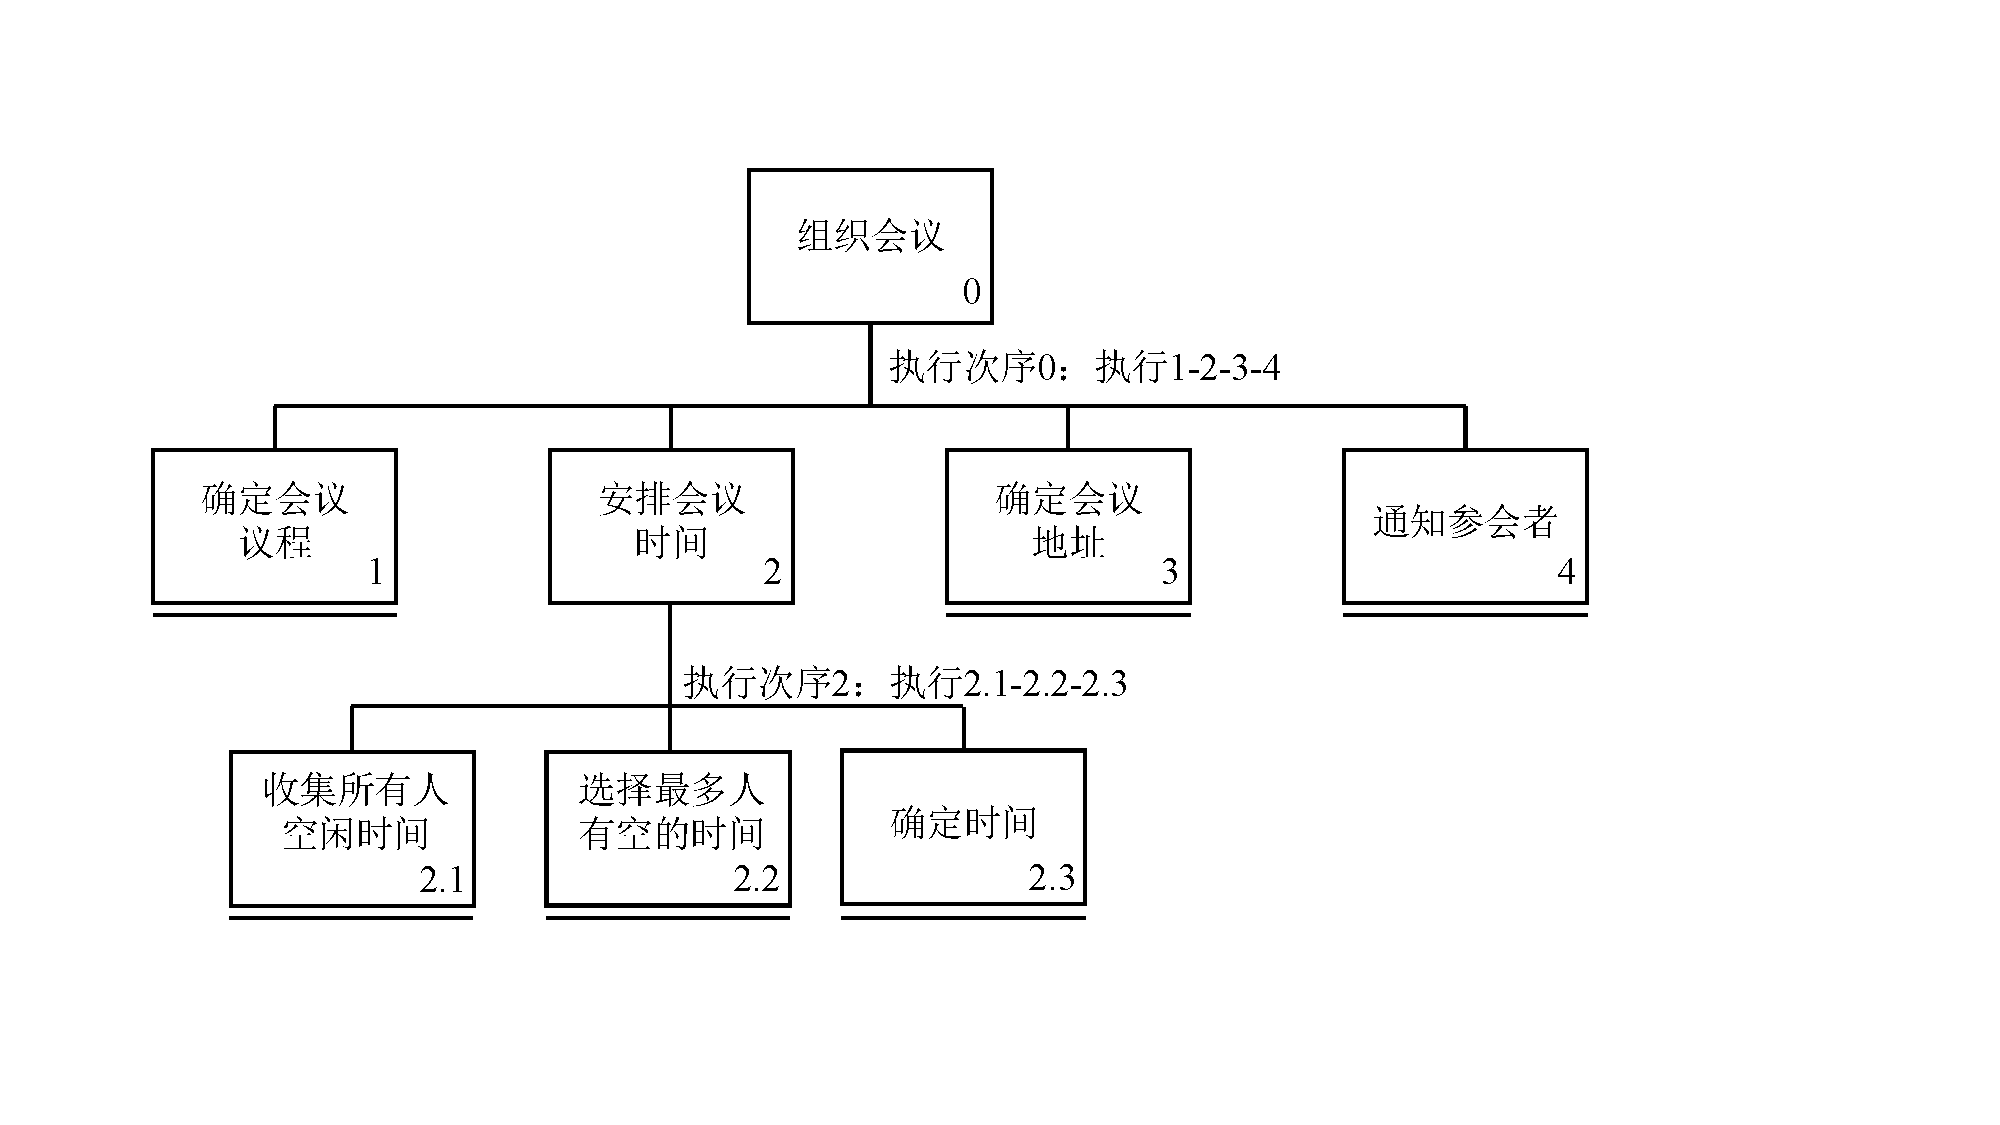
\includegraphics[width=0.63\textwidth]{3.pdf}
    \vspace{-1em}
\end{figure}
\end{solution}



\begin{problem}
为下列每一种情况选择一个适当的评估方法。在每一种情况中确定:
\vspace{-0.8em}
\begin{multicols}{4}
    \begin{enumerate}[label=\arabic*.]
        \item 典型用户
        \item 应用的技术
        \item 代表性的测试任务
        \item 评价标准
    \end{enumerate}
\end{multicols}
\vspace{-1em}
\begin{enumerate}[label=\arabic*.,start=5]
    \item 实验过程(简要描述即可,不需要罗列详细测试步骤)
\end{enumerate}

具体情况包括:
\begin{enumerate}[label=\alph*.]
    \item 你有一个戏院订票系统的原型,潜在的戏迷应用它能减少在售票处前排队。
    \item 你已经设计和实现了一个新的游戏系统,在发布以前你想对其进行评估。
    \item 已经要求你开发一个存储和管理学生考试结果的系统。在实现和给出原型之前,你希望对两个不同的设计进行测试。
\end{enumerate}
\end{problem}

\begin{solution}
\begin{enumerate}[label=\alph*.]
    \item 
    \begin{enumerate}[label=\arabic*.]
        \item 评估方法:用户测试
        \item 典型用户:戏迷
        \item 应用的技术:DECIDE模式
        \item 代表性测试任务:比较新订票系统和原有订票方式的效率
        \item 评价标准:新系统订票所有时间比原有订票方式快15\%为好,10\%-15\%为普通,小于10\%为差
        \item 实验过程:让两组用户分别用新旧两种方式进行订票,记录时间,统计分析
    \end{enumerate}
    \item 
    \begin{enumerate}[label=\arabic*.]
        \item 评估方法:用户测试、用户观察
        \item 典型用户:游戏爱好者
        \item 应用的技术:边说边做、DECIDE模式
        \item 代表性测试任务:新游戏系统的可用性和用户体验情况
        \item 评价标准:对于界面,用户满意度>85\%为优,70\%-85\%普通,70\%以下为差;对于游戏情节设置:响应时间为优
        \item 实验过程:安排用户学习体验游戏系统,可在过程中有道用户说出自己想法,并进行记录。之后发放问卷调查用户体验,统计数据,分析
    \end{enumerate}
    \item 
    \begin{enumerate}[label=\arabic*.]
        \item 评估方法:专家访问
        \item 典型用户:教务人员老师
        \item 应用的技术:问卷调查、访谈
        \item 代表性测试任务:了解用户对于两个设计方案的看法,并进行比较
        \item 评价标准:在不同的方面分别进行比较,用户满意度高的优
        \item 实验过程:安排用户在一个安静的环境中,将两个设计方案向用户描述,听去用户建议,再发放问卷,对不同方面进行调查,统计数据、分析
    \end{enumerate}
\end{enumerate}
\end{solution}






\end{document}

